% This is lnbip.tex the demonstration file of the LaTeX macro package for
% Lecture Notes in Business Information Processing from Springer-Verlag.
% It serves as a template for authors as well.
% version 1.0 for LaTeX2e
%
\documentclass[lnbip]{svmultln}
%
\usepackage{makeidx}  % allows for indexgeneration
\usepackage{graphicx}
% \makeindex          % be prepared for an author index
%
\newcommand{\ale}[1]{}%\footnote{ALE: #1}}
\newcommand{\mari}[1]{}%\footnote{MARI: #1}}
\begin{document}
%
\mainmatter % start of the contribution
%
\title{Prototypes are forever\\
  Evolving from a prototype project\\ to a full-featured system}
%
\titlerunning{Prototypes are
  forever} % abbreviated title (for running head)
% also used for the TOC unless \toctitle is used
%
\author{Hugo Corbucci\inst{1} and Mariana V. Bravo \inst{1} and
  Alexandre Freire\inst{1}}
%
\authorrunning{Hugo Corbucci et
  al.}  % abbreviated author list (for running head)
%
%%%% list of authors for the TOC (use if author list has to be
%%%% modified)
\tocauthor{Hugo Corbucci and Mariana V. Bravo and Alexandre Freire da Silva}
%
\institute{Agilbits, Sao Paulo, Brazil,\\
  \email{{hugo,marivb,freire}@agilbits.com.br}}

\maketitle % typeset the title of the contribution
% \index{Ekeland, Ivar} % entries for the author index
% \index{Temam, Roger} % of the whole volume
% \index{Dean, Jeffrey}

\begin{abstract} % give a summary of your paper
  Prototypes are a well known, widely accepted development practice
  but, if not carefully evolved, they can become a little nightmare to
  maintain. This paper presents the experience of a four people agile
  team who successfully grew a new prototyped system to a
  full-featured software system without any clear transition in the
  project. The paper describes how the project started with a very
  simple prototyping goal, evolved through iterations and spikes to a
  partly working system and transformed, in the end, in a complete
  application widely tested and refactored.

  % please supply keywords within your abstract TODO Keywords
  \keywords {prototype, agile methods, refactoring,  }
\end{abstract}
%
\section{Introduction}

Prototyping is an activity that most developers have heard about. Fred
Brooks mentioned it in The Mythical Man-Month~\cite{Brooks1975} as one
of the best ways to provide a quick view of a feature to the clients
or users to help them make a choice. Dynamic System Development Method
(DSDM)~\cite{DSDM} is heavily based on prototyping and other agile
methods also adopt many ideas related to this concept like
spikes~\cite{XP} in the Extreme Programming exploration
phase.

Successful software prototypes look very much like complete features
given a certain execution path. Therefore it is common that the
customers are so satisfied that they want to integrate the prototypes
to the working system and move on. The problem is that prototypes are
frequently created in a ``quick and dirty'' fashion and the result is
not adequate to be incorporated in a full-featured system. Yet it is
quite hard to explain this fact to the stakeholders who usually do not
want to invest any more money in this ``already working'' feature. The
consequence is that they switch priorities, focus developer work
efforts on other parts of the system and leave the rough prototype
lost within the code base. Months or years later, the prototype has
become a part of the system but is filled with bugs, unhandled corner
cases and, frequently, crappy code. Nobody remembers what it was
supposed to do or whether it is really important. Maintainability gets
deeply affected and developers get that natural and unpleasant
I-told-you-so feeling. %TODO trauma?

Developers that have been through the pain of maintaining those dirty
prototypes are no longer enthusiastic to work with prototypes. If they
have to, they make it so that there will be absolutely no way to
integrate the prototype to the existing system by either using a
different platform, language or even creating prototypes in other
medias. That inflexibility can reduce the ability of responding to
changes quickly and therefore harm the clients' interests.

This paper presents how a four-people collocated team managed to start
a prototyping project and evolve it naturally to a full-featured
application.  We have organized this experience report following the
chronological order of the project's evolution. Section
\ref{sec:start} will present the project as it was first introduced to
the development team. Section \ref{sec:working} presents the work
process established by the team to create the software based on
prototypes. After some time, the team felt that the customer needed a
full featured application, we describe this change in Section
\ref{sec:changes}. The following section (Section \ref{sec:adapting})
shows how the team adapted to change to evolve the prototype to a
production ready application. Finally Section \ref{sec:nowadays}
presents the current status of the project. Section
\ref{sec:conclusion} concludes with a summary of practices that were
useful to go through this experience without much pain.

\section{Starting the project}
\label{sec:start}

Back in March 2008, our company was hired to do some consulting for
one of the largest movie producing companies in Brazil. The client had
a great idea for a software to write movie scripts but had absolutely
no knowledge about software development.  He wanted to mature the idea
and understand how much investment it would take to turn it into
working software in order to establish his business plan. The
company's job at the time was to scout the market, discover
competitors and provide an estimation of the work needed to develop
the client's idea.

For such work, one consultant was assigned to understand what were the
client's needs and desires and two developers were asked to analyze
the existing script writing programs and evaluate the possible
development paths. After about 3 weeks of consulting and studies, the
team handed a deck full of story cards with two estimates each, based
on the use of two possible platforms. The first platform was an
existing open source software with several features and a copy-left
license; the second one was an Eclipse Rich Client Application
developed from scratch using Eclipse's open source framework.

This initial estimation suggested that a four people team dedicating 4
daily work hours to the project would be able to build a working
prototype of each feature described in about nine months of
development using the existing open source software and about one year
using Eclipse's platform. The open source solution had the advantage
to provide full functionality of several other features. For a
complete system, the estimation was well over 2 years of work on the
Eclipse version and about a year and a half for the open source one.

After some discussion, the client opted for the Eclipse based solution
due to the license restriction of the open source one which conflicted
with his business plan. He also chose to develop only a prototype of
the idea since 2 years seemed like a too heavy investment for him
alone.

After the exploration phase, the consulting contract ended and a new
negotiable scope contract~\cite{XP}
with emphasis on development effort was established. This new contract
established a team of 4 developers working with open scope that would
be negotiated monthly, providing 160 hours of work each month. It
specifically stated that the developers would work on pairs all the
time and that the developed system should have automated tests to the
production code.

% Initial priority of the stories, taken from Paulo's spreadsheet:
% Phase 1 => read TXT / separate and number act, sequence and scenes /
% read and show touch / read and show "thread" (characters) / "vision"
% (script tree) / zoom / add notes (summary) / edit touch and
% "threads" Phase 2 => create script from scratch / edit script text /
% "mundo das fichas" Phase 3 => read RTF / read and export FDR

The features initially presented to the team were grouped by the
client into 3 priority groups. The first group contained all features
most critical to the client, the ones that would allow him to
experiment with his ``big idea''. The second one comprised of some
features already present in most script editors in the market, such as
editing the script text itself. Most features in this second group
were in fact epics. The third group contained only features to read
and export to different file formats, such as those used by competitor
programs.

The project's goal was to create a high visual fidelity prototype with
mostly faked or simplified features from the first group. The client
would use this prototype to present his ideas to investors by October
2008. This meeting would either boost the project's development to a
full featured system if the investors liked the idea or end its
development in case they rejected it.

That was the team's vision of the project when the development
begun. A short seven months project whose fate would be decided by its
capacity to impress investors. Therefore, the main goal was to provide
support for the client's demonstration to ensure the project's growth
and success. The next section (Section \ref{sec:working}) describes
how the team organized itself to achieve this goal.

\section{Prototyping phase}
\label{sec:working}

Given the project's objective, the customer always prioritized new
features considering only one specific usage scenario. This meant
that, for most features, there were several cases which the team was
asked \textbf{not} to handle. Regarding the source code, it meant that
no verification or validation was written and the prototype would
crash if the user did not behave as expected. We also incorporated
several spikes as permanent solutions and did not handle a fair amount
of exceptions, ignoring errors.

The team knew since the beginning that the client would change his
mind over time. After all, it was partly to better understand his idea
and its applicability that he wanted to build this prototype. This
meant that features would be developed to later be thrown away while
code produced only for a quick spike was going to become part of the
system. Therefore, since the beginning the team invested on design,
automated tests and refactoring, just enough to keep the system
flexible to receive the next changes. The team also made it clear for
the client that he would need some work done on features after he
accepted them in order to polish the work.

Since the start, the team installed a continuous integration
server\footnote{http://www.jetbrains.com/teamcity/ - Last accessed on
  27/02/2010} to automatically build a new version of the system
hourly. This way, the client could follow the system's evolution, test
the features and provide feedback within a very short time span. This
allowed for absolutely no surprises on review meetings and improving a
lot the team's ability to tune each feature as they were released.

The first few iterations went quite smooth, developing features from
the first phase which involved importing a script in a text-only
format, providing a simple way to mark text with meta-data and a way
to manipulate and visualize this data. For these first features, it
was easy to avoid inconsistencies since there were not many business
rules involved.

Meanwhile, the client's demonstration script was evolving as the
prototype did and the team was able to use conditionals as needed to
ignore cases he would not enter in during his presentation to
investors. By October 2008, the main features from the first group
were ready for demonstration, although not finished and polished for
real use. However, by testing and playing with these features, the
client felt that the program lacked an important aspect of script
editing programs, which was the text editor itself. It was an epic
initially included only in the second group of features, but he wanted
to see how the text editor would integrate to allow viewing and
editing of the meta-data he was creating. Therefore, he prioritized
the inclusion of an incipient text editor in the prototype and started
to detail stories related to this editor. As a result of this
discovery, the client did not feel completely confident to present the
software to the investors; even so, he started to make contact with a
few people to schedule a meeting to December 2008. That date became
our new deadline until which all efforts should be focused on making a
prototyped text editor available for the demonstration.

At this point, the pressure for polishing the new features increased
since the project's fate would be decided at the demonstration and it
was close! The customer wanted the team to ignore corner cases, speed
up delivery and ensure the demonstration would run smoothly. The
excitement from the important presentation to other people (only our
one client and us had seen the software so far) was a strong
motivation for the development team to deliver all features the client
had asked for. Yet, despite unit testing and pair programming being
mandatory rules on the team, the general will to quickly deliver the
features decreased the code quality considerably.

From a development perspective, code quality was decreasing but since
the client's satisfaction was still high, there was little that could
be done.  However, external interference was about to change a bit the
situation. Section \ref{sec:changes} will explain how the project got
affected and what new direction those changes pointed to.

\section{Changing the rules}
\label{sec:changes}

December 2008 came and went without any meeting. The company that the
client was in contact with had just been acquired by another one so
any project presentation was useless until things settled down. This
relieved the team of the pressure of the upcoming deadline and we
finally acknowledged the burden of unhandled technical debt. All
members of the development team agreed that the code was getting
complex and the quality was decreasing which was affecting
productivity and speed. This combined nicely with the client's request
for a more complete text editor, with less mock-ups and
simplifications. The first iteration of 2009 was dedicated entirely to
refactoring the prototyped editor we had so far, and the iterations
that followed further developed this editor to include more business
rules.

Although the meeting with investors was mentioned in this period,
again it did not take place. The general feeling the development team
had was that the project was no longer aimed at a simple presentation
to investors. It was softly switching to a more elaborate end-user
oriented application. This seemed to be confirmed by two important and
concomitant changes that happened between June and July 2009.

In that period, the client was asking for a much more complex and
full-featured text editor and, at the same time, was exploring and
wanted to develop new features as an evolution and complement to his
previous idea. At this point, the client started to understand the
dilemma that the developers had felt so far.  How to keep a good
rhythm of new feature delivery and still cover most use cases of
existing features?

The team estimated that to have an editor with the more complex
functionality expected by the client would take at least three full
iterations. He did not welcome this news, since it would mean that no
new features would be added for a while and he wanted to explore them
with the investors' meeting still in mind.  We then decided to
investigate other possible solutions to the text editor instead of
just developing from scratch. After some research we discovered an
open source Eclipse Rich Client WYSIWYG (What You See Is What You Get)
HTML editor\footnote{\url{http://onpositive.com/richtext/} - Last
  accessed on 20/02/2010}. The editor relies on a reimplementation of
Eclipse's \texttt{StyledText} component which is responsible for
rendering text within Eclipse editors. This component was close enough
from the one we needed to implement, having some of the functionality
our client wanted on our application, and was mostly maintained by one
Russian company. So, we suggested the possibility of outsourcing the
development of the underlying text editor infra-structure to this
company, thus enabling us to continue working on the new features the
client wanted. He accepted this idea and this was the first change
that confirmed the shift towards a more full-featured system.

At the same time, the team learned that the client had formed a
dramaturgy experts group to help him better understand how to
structure the application, the existing features and the new ones. The
software was now going to have a set of beta testers and it needed to
perform decently to allow the users to suggest improvements for
it. However, the current development approach would not be able to
support this new use of the system. The change had to be clear to the
client so that development efforts would be directed to address this
new way of working. The evidence of the software's deficiency came
quickly from the dramaturgy study group. They started having trouble
with several known and unknown corner cases, unexpected behaviors and
just plain old bugs. The client recognized this problem and, despite
the fact that it would mean new features delivered more slowly,
decided it was time to invest more in usability and user
experience. This was the second change that confirmed the shift in the
project's purpose.

Meanwhile, the development team was concerned with the increasing
complexity so they started to track some data from the source
code. The first metrics was the amount of \texttt{FIXME},
\texttt{TODO} and \texttt{XXX} marks in the code. Since the beginning,
the development team added those marks everywhere they felt a corner
case or a behavior existed but was not handled. Each mark had a small
comment associated and the kind of the mark determined the critically
of the problem. Figure \ref{fig:TODOs} shows the evolution of those
marks during the project.

\begin{figure}[hbt]
  \centerline{
    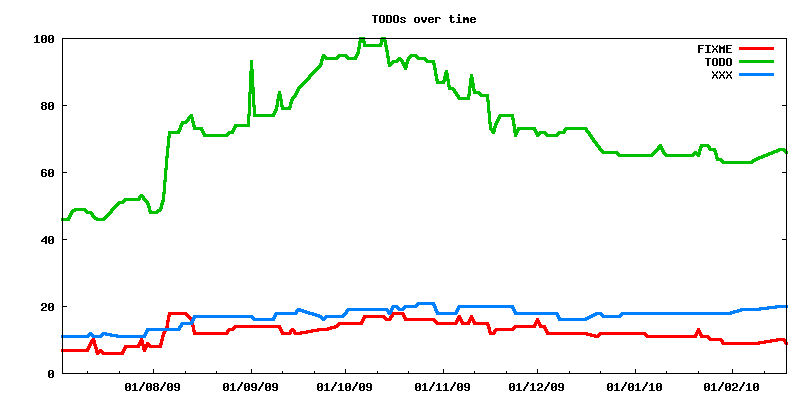
\includegraphics[width=120mm]{TODOs.png}
  }
  \caption{Evolution of FIXME, TODO and XXX marks in the source code}
  \label{fig:TODOs}
\end{figure}

It is noticeable that the first data collection of those marks is
dated for mid July 2009. It took the team some time to consider this
metric was important enough to be automatically tracked. To
consciously acknowledge that the team needed to track complexity was
step one to adapt to the new direction. The next section will present
other practices that allowed us to handle this shift.

\section{Adapting to the new rules}
\label{sec:adapting}

While the amount of \texttt{TODO} marks was fairly high, the team
still had to develop new prototyped features and therefore they
accepted to just track it and try to keep it under control. While this
gave the team some idea of code complexity, it did not help in showing
if this complexity was being tamed by tests.

By the beginning of August 2009, the client decided that it was
important for him to be able to see the evolution of the work done by
the Russian team and he decided to have two editors available on the
application. The first one was Eclipse's original one and the second
one was based on the new outsourced component. At this point, a major
code duplication was performed since features available on Eclipse's
editor were supposed to be also available on the new editor and the
goal was to eliminate the older one. The result was a huge increase in
the marks tracked as well as an increase in lines of code and the team
suspected tests were not following. A very simple script was written
to count the lines of production code and test code. Figure
\ref{fig:LOCs} shows how both metrics evolved over time. It starts at
the same date as Figure \ref{fig:TODOs} to facilitate comparisons.

As with the \texttt{TODO} metric, the lines of code showed the team a
little issue regarding testing but it was not addressed
immediately. It was well known that the code was not highly covered
since there were no User Interface (UI) tests and quite a few features
were related to the way data was shown to the user. However, the team
had a feeling that the effort to test the controller and model would
have produced more test than code.

\begin{figure}[hbt]
  \centerline{
    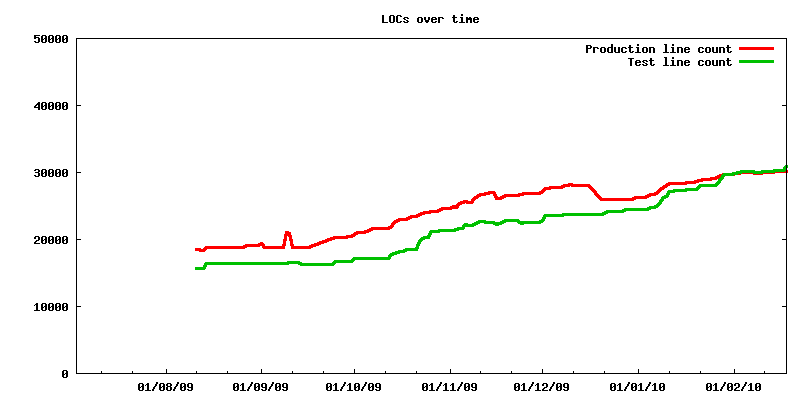
\includegraphics[width=120mm]{LOCs.png}
  }
  \caption{Evolution of production lines of code and test lines of
    code}
  \label{fig:LOCs}
\end{figure}

By this time, the customer started to mention the presentation to the
investors again. It had been quite some time in the project now and he
was feeling he had spent enough money and needed some external
investment. Therefore the old investor meeting pressure installed
itself within the team and the deadline was, again, the end of the
year. The goal was to quickly integrate the outsourced component and
tune a few features to the so expected meeting.

By the time the team understood the outcomes of those issues, the code
had reached a critical situation. \texttt{TODO} marks were amazingly
high and distance between tests and code was at its higher level. The
work was being roughly divided in three: fixing bugs, implementing new
features and integrating the outsourced component. By this time, the
team also suffered the loss of a member who was required in a full
time consulting work. The team went from two pairs to one pair and an
extra person and the velocity decreased.

Figure \ref{fig:InstanceOfs} shows yet another complexity tracker
developed by the team. Counting the amount of \texttt{instanceof} Java
reserved word led the team to understand the level of special cases
unfactored in the code. Although Eclipse's framework required a few of
those, some of them were avoidable and the team felt reducing this
number would lead to a more factored code.

\begin{figure}[hbt]
  \centerline{
    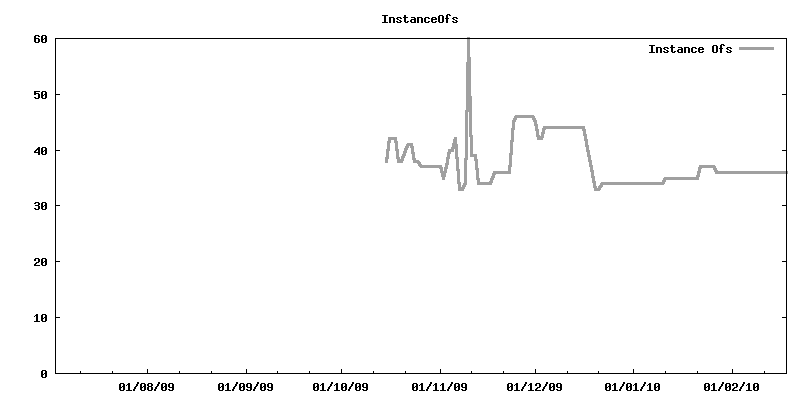
\includegraphics[width=120mm]{InstanceOfs.png}
  }
  \caption{Evolution of instanceof in the code }
  \label{fig:InstanceOfs}
\end{figure}

Curiously, as for the two previous metrics, the effect of tracking the
number of \texttt{instanceof} was not immediate. More interestingly
than that, in a short time span, having the metric did not stop it
from getting worse. In the rush to produce the features, the team was
becoming reckless with code quality.  Something had to be done or the
project was going to become impossible to maintain and the client's
demonstration would surely suffer from it.

With three persons working by the end of the year to match a two pairs
velocity and reducing complexity, the team had to calm down, step back
and rethink about agile values. Section \ref{sec:nowadays} presents
the resolutions the team adopted and their impact on the current
version of the system.

\section{Current status}
\label{sec:nowadays}

December arrived and it was time to accept a full integration of the
outsourced component and a throw away of the team's first
solution. Along with this came a serious decrease in \texttt{TODO}
marks, \texttt{instanceof}s and lines of production code as a
considerable duplication was erased. By that time, the team was
largely working with just two persons pairing full time since the
third developer was involved in other projects and hardly managed to
pair up with any of others.

The team decided it should profit from that fact and decided to
institute a merciless refactoring policy. No matter how small or how
big the refactoring was, it had to be done and it was to be included
as a regular part of each task and not as a separated task. Corner
cases were not to be left unhandled and any unsupported work was to
log its execution to the application error log. The impact of those
policies was fairly clear by the end of the month. All metrics had
improved and more bugs were being listed by the development team.

The month passed and no meeting was scheduled. The famous deadline
was, once again, a myth. With code quality increasing, \texttt{TODO}
marks decreasing, test code improving and bugs being caught by the
development team (instead of the users), the team felt an extra
developer would help increase velocity and so started to train one to
join the team in January. With the insertion of this new member in the
team, some work was performed on another platform which led to the
discovery of a series of platform specific bugs. The general feeling
was that the client was getting ready to wrap up the project since he
was quite happy with the software and was considering he invested too
much already on this idea.

However, in the next meeting, the client presented an officially hired
beta tester that was going to support the team in order to improve the
usability of the system. They also presented the team with a load of
new features and usability improvements that they wanted to have
done. The client also mentioned that he was thinking seriously about
dropping the quest for investors and releasing the product by
himself. In order to do so, bugs needed to be eliminated. Any bugs
found immediately gained the highest priority and should be solved in
some way as soon as possible.

With this new policy, the beta tester started to find problems with
the existing features because some business rules were
contradictory. The issues reported to the customer led him to study
and analyze his business model better and the rules evolved. Thanks to
the experience that the client had accumulated so far in the project,
he allowed himself to experiment with a few solutions until he felt
more comfortable with the way features worked, allowing him to seek
consistency, conceptual integrity and the certainty that other choices
were not as good as the one he had made.

\section{Conclusion}
\label{sec:conclusion}

Successful software prototypes need not always be completely thrown
away. This fact comes from the very nature of software and the ability
to easily and quickly merge pieces of code together to produce a
working system using agile methodologies. Agility relies on this fact to allow for incremental
evolution of the system and, therefore, supports that drafts should
grow to complete features.

By embracing that, if your prototypes are successful, they will be
incorporated into the software, but you have to prepare to maintain that
code. It does not mean that prototypes should be developed exactly
as well known complete features. Prototyping should allow you to
explore different solutions and as they survive
the selection process they should be refactored and evolved in a similar fashion to the set-based lean approach~\cite{Poppendieck2009}.

Refactoring, testing and decoupling are essential to allow code
evolution and should be practices that are strongly enforced as the prototype 
starts to transform into a working feature. 
Unhandled exceptions, cases or behaviors should be
documented with tests or some other system that allows for
quick listing and search.

Although prototypes are not first class production code and much of
their value comes from this lower class status, they are likely to
climb the ladder up to working essential features of the system. It
is very important to track this evolution and provide the necessary support
to maintain quality. Even so, do not fear to throw away anything either,
the value provided by prototypes resides deeply in the knowledge they
brought to the customers which means the code is much less valuable
then we give it credit for. In our experience using prototypes to test out different ideas for the same feature proved invaluable, and many accepted prototypes were able to evolve to production code in the application.

%
% ---- Bibliography ----
%
\begin{thebibliography}{5}

\bibitem{Brooks1975} Brooks Jr., F.P.: The Mythical Man Month: Essays
  on Software Engineering. Addison-Wesley (1975)

\bibitem{DSDM} DSDM Consortium: DSDM: Business Focused
  Development. Addison-Wesley (2002)
  
\bibitem{XP} Kent Beck and Cynthia Andres: Extreme Programming Explained: Embrace Change, 2nd Edition. Addison-Wesley (2004)  

  % ale: achei que era uma boa ter mais referências sobre
  % prototipos. eu tirei essa história de prototipos de alta
  % fidelidade visual ou alta fidelidade funcional de uma apresentação
  % que vi sobre UX e prototipagem de interface lá na locaweb, no
  % scholar.google achei isso aqui:

  % http://74.125.155.132/scholar?q=cache:ezGZKBBRVhwJ:scholar.google.com/+software+prototype&hl=pt-BR&as_sdt=2000

  % http://www.imamu.edu.sa/Scientific_selections/abstracts/Documents/A%20Systematic%20Look%20At%20Prototyping.pdf

\bibitem{Poppendieck2009} Poppendieck, M. and Poppendieck, T.:
  Implementing Lean Software Devleopment: From Concept to
  Cash. Addison-Wesley (2009)

\end{thebibliography}
%
\end{document}
